% !TeX root = ../../main.tex
% 第一章 井筒深度清洁技术研究现状与总体技术路线
% 素材来源：《9-5/8"井筒深度清洁关键技术升级研究》调研部分（研究背景、研究意义、技术路线、21 项工具调研）

\chapter{井筒深度清洁技术研究现状与总体技术路线}\label{chap:survey}

\section{研究背景与意义}

井筒清洁是贯穿钻井、完井、修井与生产全过程的共性工序，其任务是清除套管内壁附着的钻井液泥饼、水泥环残渣、射孔毛刺、铁锈氧化皮、结垢物与蜡质，以及磨铣、套铣、刮削等作业产生的金属碎屑。井筒清洁不彻底，轻则造成筛管堵塞、封隔器胶筒划伤与坐封失效，重则引起下部完井管柱遇阻坐挂失败、上部完井管柱插入密封不到位、油管挂锁紧失败、采油树内树帽无法到位等复杂情况，并造成储层污染。统计表明，完井与修井作业中约 30\% 的非生产时间（NPT）与井筒清洁问题相关。

影响清洁效果的因素包括钻井液的流型与流变性、岩屑下滑速度、环空返速、钻杆转速与往复运动、井筒尺寸与井斜、管柱居中度以及碎屑的尺寸与形状；在井径突变处与工具的几何变径处易形成环流死角，成为碎屑沉积的“危险位置”。需清除的碎屑可归纳为砂砾、结垢物、铁屑、蜡质等，其密度、形状与黏附性差异极大，单一清洁机理难以全面覆盖。海上深水井的矛盾更为突出：受日费与作业窗口制约，要求一趟管柱同时完成生产套管、隔水管与防喷器的清洁，并要求起钻时把碎屑带出井筒而不是循环回井内。%核实

与上述要求相比，国内修井工具长期依赖进口，斯伦贝谢、贝克休斯、威德福等公司占据大部分市场份额；国产工具在寿命、效率、功能性与可靠性上与国际领先水平仍有差距，且国内尚基本没有成体系的工具性能测试装置，工具的清洁效率、通过性与寿命缺乏可对比的量化评价手段，难以支撑工具的持续迭代。

针对上述问题，本项目以 9-5/8\inch 井筒为对象开展深度清洁关键技术升级研究，主要内容包括五个方面：一是模拟砂砾、铁屑、结垢物与蜡在不同流速、粘度条件下的运移与分布规律，并开展室内实验验证；二是调研高强与高温磁性体的性能，筛选最优产品，优化磁路布置规律与安放位置，分析消磁因素；三是建立水力脉冲模型，分析脉冲频率对井壁清理与携屑能力的影响；四是模拟刮板在不同弹力下的清洁效果并给出最优弹力分布，模拟钢刷材质与钢丝长度并给出最优组合；五是开展工具应用效果主控因素的识别研究，通过相关性分析确定显著参数。为此，需先厘清国内外井筒清洁工具的技术现状、优势与局限，明确本项目的技术切入点。

\section{国外井筒清洁技术研究现状}

国外在井筒清洁工具研发方面投入较大，创新成果丰富，已形成“按清洁机理分类—工具系列化—系统集成化—实验验证配套”的技术体系：机械、物理与化学三类清洁工艺各有专用的工具与材料，三大油服公司再把刮削、刷洗、磁吸、过滤与循环控制做成可自由组合的模块，按井况配套成一套管柱，并依托专用试验装备持续迭代。

\subsection{机械清洁工艺与工具}

机械清洁依靠刮刀、刃片与刷毛对套管壁面施加机械作用，清除泥饼、水泥残渣、锈斑与结垢。近年来国外的改进集中在两个方面：一是刮刀结构与材质的优化，通过改变刃口几何形状并选用耐磨材料，使其更好地适应不同硬度的污垢与套管壁材质；二是驱动方式的升级，部分新型旋转刮管器采用电机驱动系统，可精确控制刮刀的旋转速度与压力，以应对复杂多变的清洁需求。机械类工具的共同优点是作用力直接、对硬质垢与水泥环残渣清除效率高、作业过程可控；不足是刃片与套管壁直接接触，存在划伤套管与遇卡的风险，且对胶皮、蜡质等软质附着物效果有限。

\subsection{物理清洁工艺与工具}

物理清洁以流体能量或声能剥离污垢，主要包括高压水射流清洗与超声波清洗。高压水射流工具的进步集中体现在喷嘴技术上：通过设计特殊形状与内部结构的喷嘴，使射流能量分布更集中、更均匀，从而大幅提高清洗效率，空化射流与脉冲射流即由此发展而来。超声波清洗的进展则体现在换能器性能上：采用新型压电材料制作换能器，提高了超声波的转换效率与振动强度，清洁效果随之增强。物理类工具的优点是不依赖刃口、不会划伤套管，可进入缝隙与孔洞；不足是需要较高的泵压或电功率，对厚垢、水泥环与金属碎屑的清除能力有限，且只能松动污垢而难以把碎屑带出井筒。

\subsection{化学清洁工艺与清洗剂}

化学清洁通过清洗剂溶解或分散特定类型的污垢。国外近年研发出多种针对性强、环保性能更好的化学清洗剂，通过对成分与配方的优化，使其能够更有效地溶解蜡质、盐垢、泥饼等特定污垢，同时减少对井筒材质的腐蚀和对环境的污染。其优点是作用均匀、可覆盖射流与机械工具难以触及的部位；不足是作用时间长，需与钻井液体系配伍并对返排液进行处理，对金属碎屑与水泥块等固相无效，单独使用难以满足完井阶段的清洁要求。

\subsection{三大油服公司的集成化清洁系统}

国外三大油服公司已把上述单一机理的工具发展为成套系统，形成“工具系列化、系统集成化、实验验证配套”的格局。

斯伦贝谢的 Wellbore Cleaning System 以多功能集成为特征，追求一趟完成刮削、清洗与碎屑回收。BRISTLE BACK 套管刷以高强度刷毛配合非旋转稳定器套筒，在减少套管磨损的同时适配多种井径；MAGNOSTAR 强磁工具以强磁场捕获磁性碎屑，适用于深水与高温高压井；RISER MAGNO BUCKET 可在较低环空返速下捕集大颗粒，正反循环均可工作，高温高压下性能稳定。其优点是集成度高、单趟作业效率高、可显著降低非生产时间；不足是结构复杂，价格与配套服务门槛高，各部件对井况的适应性边界仍依赖服务商的经验判断。

\textcolor{red}{哈里伯顿的 RZR 系统走模块化路线。RAZOR BACK 套管清洁工具以 360° 金属刃片实现均匀的清洁力，刃片柔韧性好，遇卡风险低；VACS 文丘里工具借助文丘里效应产生较大吸力，无需复杂动力即可工作，能自适应井斜，并可与其他模块及化学清洗协同。其优点是组合灵活、可按井定制、模块可重复利用；不足是模块数量多，现场组织与判断要求高，组合不当会相互干扰。}

贝克休斯的 Wellbore Cleanup Tools 侧重高强度与深水高压适应性。PUP RISER BRUSH 采用三环不锈钢刷圈，清洁效率高而压耗低；DUAL-ACTION BYPASS SUB 为双向往复循环阀，高强度材质适应深水高压工况，并可按井定制。其优点是承载能力与可靠性好；不足是单项功能相对单一，仍需成串配套使用\footnote{姚：dual action bypass sub的功能是什么；缺少工具的图片}。

三种技术取向可概括为：斯伦贝谢重多功能集成，哈里伯顿重模块化组合，贝克休斯重高强度与深水适应性，其共同点是把单一工具做“专”，再靠系统集成覆盖全部碎屑类型。

\subsection{国外典型工具的技术特点}

\textcolor{red}{工具图片！}

除三大油服公司外，国外专业工具厂商近年推出的几款一体化工具也代表了相关技术方向。CHIMERA 一体式刮削器以整体式刮削笼与扶正器单体坯料直接加工成型，取消了弹簧、螺栓与垫片等易失效件，采用非旋转设计并配轴向—径向复合的合金青铜轴承，耐高温且耐化学腐蚀，可选配镶焊碳化钨的一体式管柱铣刀，兼容各类 API 与优质钻杆扣型；重型版带管柱铣刀、标准版为光滑外径，到达坐封深度后旋转并在关键深度往复三次以上。其优点是以结构简化换取可靠性；不足是整体式结构不可局部更换，损坏后需整件替换，使用成本高。

INNOBRISTLE 完井尾管通井清洁工具把通井与清洁并入完井管柱：底接头外径略大于封隔器以确保井眼畅通，实心钢底接头承重且可回收，并内嵌碎屑收集磁铁；柔性钢刷在封隔器胶筒激活前即时通过，专门清洁封隔器密封区，另可配封闭顶接头与自对准引鞋，下压即可旋转 180°。其优点是随完井管柱同步通井、流体旁通面积大；不足是专用性强，只适用于完井尾管通井工况。

X-Treme Clean XP 套管刮削器采用无内部连接的一体式心轴，抗拉抗扭强度高于钻杆接头，允许转速达 150 r/min，内径与环空流通面积大；刀片为新型螺旋结构，双面及端部协同刮削，刮削面积达常规工具的两倍以上，非旋转刀片配扶正器以防止套管磨损，适用于深水、深井与斜井。与之配套的 X-Treme Clean XP 井下磁力打捞器采用高温强化磁体与创新的磁极排列，捕获与携载能力达常规工具的数值，高温高压下性能稳定；磁棒组可更换以实现模块化维护，磁极间隙经优化使碎屑吸附于磁棒间隙而不占用循环通道，双端稳定器提高斜井居中度，同样支持 150 r/min。这两类工具的共同优点是强度储备高、可与高速旋转作业兼容；不足是加工精度要求高，价格明显高于常规工具。

\subsection{国外工具性能测试装备}

国外工具之所以能够持续迭代，很大程度上得益于配套的试验装备。NOV 的 HMM 卧式铣床可模拟大斜度、水平与常规套管工况，最大扭矩 41 kN·m，最大机械钻速 61 m/h，最高转速 140 r/min，并配有数据采集系统；此外还有猫道、震击等专用测试设备与工具试验井。相比之下，国内同类试验能力基本空白，这也是国产工具性能数据难以横向对比的根本原因。国外典型工具与系统的优缺点汇总见表 \ref{tab:foreign-tools}。

\begin{table}[H]
	\centering
	\caption{国外典型井筒清洁工具与系统的优缺点对比}
	\label{tab:foreign-tools}
	\footnotesize
	\renewcommand{\arraystretch}{1.3}
	\begin{tabularx}{\textwidth}{@{}>{\raggedright\arraybackslash}p{3.2cm}>{\raggedright\arraybackslash}X>{\raggedright\arraybackslash}X>{\raggedright\arraybackslash}p{2.6cm}@{}}
		\toprule
		工具/系统 & 主要优点 & 主要缺点 & 适用井况 \\
		\midrule
		X-Treme Clean XP 套管刮削器 & 一体式心轴强度高于钻杆接头，允许 150 r/min；螺旋刀片双面与端部协同刮削，刮削面积为常规工具两倍以上，非旋转刀片配扶正器防磨 & 加工精度要求高，价格高，刀片磨损后需返厂处理 & 深水井、深井、斜井 \\
		CHIMERA 一体式刮削器 & 整体式刮削笼与扶正器一体成型，取消弹簧、螺栓与垫片；合金青铜轴承耐高温、耐化学腐蚀 & 整体式结构不可局部更换，损坏后需整件替换 & 高温高压井、含化学药剂环境 \\
		INNOBRISTLE 尾管通井清洁工具 & 通井与清洁并入完井管柱，柔性钢刷专清封隔器密封区，底接头内嵌碎屑收集磁铁 & 专用性强，仅适用于完井尾管通井，单件功能少 & 完井尾管、封隔器坐封前 \\
		X-Treme Clean XP 井下磁力打捞器 & 高温强化磁体与优化磁极排列，捕获携载能力达常规数倍；磁棒组可更换，双端稳定器提高居中度 & 仅对铁磁性物质有效，对胶皮、泥饼与岩屑无能为力 & 高温高压井金属屑回收 \\
		高压水射流与超声波清洗工具 & 不以刃口接触套管，不划伤管壁；喷嘴与换能器改进后能量更集中，可进入缝隙孔洞 & 需高泵压或大功率电源，只能松动污垢，难以把碎屑带出井筒 & 结垢、泥饼与近井带处理 \\
		化学清洗剂 & 配方针对性强、环保性能好，可溶解蜡质、盐垢与泥饼，覆盖工具难以触及的部位 & 作用时间长，需与钻井液配伍并处理返排液，对金属屑与水泥块无效 & 石蜡、盐垢与有机垢清除 \\
		斯伦贝谢 Wellbore Cleaning System & 刮削、刷洗、磁吸与碎屑回收集成于一套管柱，单趟完成，非生产时间低 & 结构复杂，成本与配套服务门槛高，适应性判断依赖服务商经验 & 深水井、高温高压井 \\
		哈里伯顿 RZR 系统 & 模块化组合灵活，可按井定制；VACS 无需复杂动力、可自适应井斜 & 模块多，现场组织与判断要求高，组合不当易相互干扰 & 多井况按需定制 \\
		贝克休斯 Wellbore Cleanup Tools & 高强度材质，深水高压下可靠；刷洗压耗低 & 单项功能较单一，仍需成串配套 & 深水高压、大载荷井 \\
		NOV HMM 卧式铣床等试验装备 & 可模拟大斜度、水平与常规套管工况，扭矩 41 kN·m、钻速 61 m/h、转速 140 r/min，具备数据采集 & 装备投资大，仅油服公司与专门机构具备 & 工具研发与性能标定 \\
		\bottomrule
	\end{tabularx}
\end{table}

\section{国内井筒清洁技术研究现状}

国内工具的发展路径与国外不同，多由现场复杂井况倒逼形成，普遍以“一项作业配一件专用工具”起步，近年才向一体化、集成化方向演进。

\subsection{整体研究态势}

国内在井筒清洁工艺及工具的研究方面已取得一定成果，但相较于国外先进水平仍存在差距。在基础研究领域，对各类井筒清洁工具工作机理与失效机理的研究深度有待加强，尚未形成完整、系统且深入的理论体系，导致工具的研发与改进缺乏精准的理论指导，多依赖经验性探索与尝试；同时，准确有效的测试方法与测试装置相对匮乏，限制了对工具性能进行全面、精确的评估，难以实现从实验室研究到实际井下应用的高效转化。

\subsection{一体化多功能清洁工具}

\textcolor{red}{中海油的 MTWF 多功能井筒清洁器把毛刷总成、旁通孔、破裂盘、碎屑回收腔与筛缝过滤器集于一身：下入时毛刷上行、旁通孔开启，以防压活塞；起出时旁通孔关闭，环空流体经毛刷上部流道进入回收腔，经筛缝过滤器后碎屑随起钻带出；\textcolor{red}{当回收腔充满或滤网堵塞时，可通过环空加压约 4.55 MPa 剪破破裂盘建立新的循环通道}。该工具在渤海 A1H1 分支水平井一趟完成刮管洗井与碎屑收集，显著降低了防砂管柱下入风险，适用于井斜大于 40° 的大位移井、环空难以提高返速及大部分深水井。其明显短板是不具备磁吸功能，细小铁屑易被漏过，需另配强磁工具。}

中海油南海深水井则采用成套工具串，包括隔水管刷、水下防喷器冲洗接头、多功能过滤器、多功能阀、可旋转刮管器、VACS 喷射短节与强磁刮管器。各件设计各有巧思：隔水管刷以上毛刷、下捞篮的组合实现无活动部件，可承 100 r/min 且毛刷不转而减少隔水管磨损；水下防喷器冲洗接头借投堵头形成锥面压差，井口打压约 8.96 MPa 剪销后滑阀下移露出水眼，实现全方位喷射；可旋转刮管器设“自由旋转态”与“解卡态”两种工作状态，正常时刀片扶正套不转而心轴高速旋转，以提高返速、降低磨损，遇卡时上提剪断剪切环使刀片与扶正套同步转动。但这套工具串的共性问题也很清楚：\textcolor{red}{每件工具专一性强、普遍适应性不足，必须组合使用，而组合越多结构越复杂、系统可靠性越低}；此外过滤器易堵，冲洗接头与多功能阀对投堵时机和控压精度要求高，VACS 喷射短节易堵且负压受深水高压削弱，强磁刮管器遇粗磨屑易桥堵。

中石化西北油田的多功能一体化工艺则把机械刮管器与磁性短节做成一体：单根一体式中心管上螺旋排列刮刀，设应急剪切销钉以便遇卡时上提解卡；磁性短节将强磁块镶嵌于本体长槽，装于刮管器上下两端。截至 2022 年 5 月累计应用 139 井次，工艺成功率 100\%。其不足同样具体：强磁块的镶嵌方式易脱落并遗落井内、难以打捞；刮刀在弹簧作用下始终贴紧套管，加剧刮刀与套管的双向磨损。改进方向已指向高强度粘结剂或机械锁定、磁性导向打捞与电磁定位回收，以及可伸缩刮刀、智能弹簧与耐磨涂层。

孟凡华等针对常规工具结构复杂、性能单一、需多次起下钻回收的问题，研制了由管柱总成、清洁总成与回收总成组成的新型多功能套管清洁工具：钢刷清洗、分流筒割缝排液、碎屑沉入回收筒；回收筒长度可按预测碎屑量增减，使极限回收量大于井筒杂质总量，从而一趟完成；设钢珠—喇叭孔的锁定开关装置，转 90° 即打开回收孔取屑；紫铜破裂盘的破裂压力为 4.14 MPa；心轴材料为 42CrMo、屈服强度 930 MPa，有限元校核在 130 t 拉力下最大应力 895.68 MPa、20 kN·m 扭矩下最大应力 865.6 MPa，均满足要求。该工具在海上 A-X1 井（水深 91.40 m、完钻井深 5050 m、224.5 mm 套管）一趟完成清洁，累计 9 井次应用均成功，并以“回收碎屑体积与回收筒最大容积之比”大于 80\% 判为尚不清洁、小于 20\% 判为完全清洁。不足是部件繁多，制造与装配精度要求高，井下故障排查与维修困难。

\subsection{刮管与刷洗工具}

\textcolor{red}{工具的作者是谁？}
旋转刮管器通过扶正套与上接头的钢珠连接、环形弹簧钢刮刀组件实现“自由旋转态”与“解卡态”两种工作状态，结构巧妙但易损件（刮刀、弹簧、钢珠）多、维修困难。超声波刮管器由超声波发生器、换能器与刮管头组成，以超声除垢与机械除垢双重作用清洁套管，单点作用 10 s 以上即可除垢，适配 5-1/2\inch、7\inch 与 9-5/8\inch 套管，结构简单坚固、操作与保养方便；但其不足也很突出：高温高压强腐蚀环境下性能受限，集成发生器导致工具尺寸与重量偏大，下入深度与操作空间受限制约，且同样不具备磁吸功能。新型套管清洁工具以中心管、毛擦、回收筒与扶正器为主体，下入时兼作打捞杯，起钻时关闭旁通、经筛管过滤介质捕捉碎屑，起出井口后打开清除窗倒出碎屑；9-5/8\inch 规格抗拉不低于 600000 lb、内径不小于 2.688 in、上扣扭矩 18900 ft·lb、筛管流动面积不小于 51.5 in$^2$，但结构复杂、制造成本高。

\subsection{磁性打捞与磁吸清洁工具}

\textcolor{red}{工具的作者？}

强磁打捞器以磁环组件配打捞杯构成，打捞杯与磁环组件的组合增强了清洁功能，可与旋转刮管器组合或单独入井；244.5 mm 规格的外径为 209 mm、内径 70 mm、长 2105 mm、抗拉 1200 kN、抗扭 25 kN·m。西北油田所用的磁性短节则把强磁块镶嵌于本体长槽内，装于刮管器上下两端，在起下钻过程中吸附铁屑。此类工具的局限由原理决定：只对铁磁性物质有效，对胶皮、泥饼、砂粒与岩屑等非磁性杂质无能为力，单独使用无法实现全面清洁；此外镶嵌式磁块存在脱落遗落井内且难以打捞的潜在风险。

\subsection{水射流与脉冲类工具}

空化射流水力振荡器把空化结构与水力振荡器相结合，借剪切空化与二次空化产生的冲击波和微射流增强振荡强度，与高压旋转射流冲洗器配合时，在 400 L/min 排量下除垢速度较传统水力振荡器提高 16.2\%。自激式水力振荡器利用附壁效应与反馈流道使射流周期性偏转，无移动部件、结构紧凑，脉冲频率最高 26.2 Hz、压力幅值最高 2.65 MPa，关键件采用耐高温高压合金，以适应埋深超过 2500 m 的储层。阻断式脉冲射流喷嘴用簧阀周期性阻断连续射流以生成高频脉冲，借水击效应增强瞬时冲击，并靠射流卷吸负压引入磨料形成脉冲磨料射流。这类工具的共同优势是能量利用率高、无活动部件、可靠性好；共同局限是依赖较高的泵压与排量，对水泥环、硬质垢与铁屑的固态回收无能为力，只能松动而不能带出。

\subsection{负压与过滤类工具}

油井井筒除垢屑过滤器以移动刮板、收集斗、清理喷头与抽吸口实现刮削—冲洗—抽吸三个过程，现场效果为石蜡垢厚度由 3 mm 降至 1 mm 以下、日产油由 10 T 升至 12 T，高含蜡井生产周期延长近 30\%，高矿化度井盐结晶减少约 80\%，但滤网易堵且存在压力损失。负压井底清洗工具利用射流负压（流速大于 30 m/s 时喷嘴出口接近真空）配旋流与过滤分离，能主动吸取粘性泥饼与重金属屑，可深入缝隙孔洞，且不受重力方向限制而适应水平井；代价是需要大功率动力源，井下密封件易损、维护成本高，清洗范围受负压影响范围限制。真空吸附器同样以顶部驱动头形成局部反循环，配岩屑收集筒与过滤筛管，吸力适应性好，但对真空泵性能依赖强，真空度受腐蚀、振动与温度影响。

\subsection{井眼净化类工具}

BH-HCT 井眼清洁工具以硬质合金齿配上下螺旋棱、叶轮、耐磨带与导流槽，形成刮削、双螺旋导流、叶轮离心与导流槽排屑的多方式协同，有效作用距离 80～120 m；岩屑床破坏器以 4145H 材质本体加螺旋结构与耐磨带，适应直井、斜井与水平井。二者的问题相似：效果高度依赖钻井液性能与操作参数（转速、下放速度、排量），参数匹配依赖经验，且制造精度要求高、成本不低。

\subsection{可变径刮管工具}

针对海上 2000～3000 m 井段内套管尺寸变化、常规刮管器需多次更换工具的问题，可变径刮管工具采用“芯轴＋弹簧＋板簧＋刮刀”结构，弓形板簧按一端固定、一端简支的梁模型设计，使工具可在 159.4～220.5 mm（7\inch～9-5/8\inch）范围内自适应变径并保持 360° 全周刮削；扶正套直径 $\phi$148 mm、刮刀直径 $\phi$260 mm、内通径 40 mm、总长 4147 mm，芯轴抗拉强度 965 MPa，刮刀材料为 20CrMnMo，密封圈耐温 180 ℃。其代价是结构复杂、制造与维护成本高，对高温与腐蚀环境敏感。国内典型工具的优缺点汇总见表 \ref{tab:domestic-tools}。

\begin{table}[H]
	\centering
	\caption{国内典型井筒清洁工具与工艺的优缺点对比}
	\label{tab:domestic-tools}
	\footnotesize
	\renewcommand{\arraystretch}{1.3}
	\begin{tabularx}{\textwidth}{@{}>{\raggedright\arraybackslash}p{3.2cm}>{\raggedright\arraybackslash}X>{\raggedright\arraybackslash}X>{\raggedright\arraybackslash}p{2.6cm}@{}}
		\toprule
		工具/工艺 & 主要优点 & 主要缺点 & 适用范围 \\
		\midrule
		MTWF 多功能井筒清洁器 & 刮管、洗井与碎屑回收一趟完成，渤海 A1H1 等现场应用成熟 & 无磁吸功能，细小铁屑漏过，需另配强磁工具 & 井斜大于 40° 的大位移井、深水井 \\
		南海深水井工具串 & 覆盖隔水管、防喷器与套管全流程，可旋转刮管器兼顾提速与解卡 & 各工具专一性强，组合后结构复杂、可靠性下降；过滤器易堵，控压与投堵时机要求高 & 深水井全套清洁 \\
		西北油田一体化工艺 & 结构简单，累计应用 139 井次、工艺成功率 100\% & 强磁块易脱落且难打捞，刮刀常贴套管加剧双向磨损 & 常规套管刮管 \\
		新型多功能套管清洁工具 & 回收筒长度可按碎屑量调整，一趟完成，9 井次应用成功 & 部件多，制造装配精度要求高，故障排查与维修难 & 海上完井套管清洁 \\
		旋转刮管器 & 设自由旋转与解卡两种状态，正常时降低磨损、提高返速，遇卡可上提剪断剪切环解卡 & 易损件（刮刀、弹簧、钢珠）多，维修困难 & 大斜度井、水平井 \\
		超声波刮管器 & 超声与机械双重除垢，单点作用 10 s 以上即可见效，结构简单、保养方便 & 高温高压强腐蚀环境下性能受限，尺寸重量大，无磁吸功能 & 5-1/2\inch～9-5/8\inch 套管 \\
		新型套管清洁工具 & 下入兼作打捞杯，起钻关闭旁通经筛管捕屑，井口开窗倒屑 & 结构复杂，制造成本高 & 9-5/8\inch 与 7\inch 套管完井 \\
		强磁打捞器与磁性短节 & 磁环组件配打捞杯，吸附力强，可与刮管器组合使用 & 仅对铁磁性物质有效，镶嵌式磁块存在脱落遗落风险 & 金属屑与磨铣碎屑回收 \\
		水射流与脉冲类工具 & 无活动部件，能量利用率高，除垢速度较传统振荡器提高 16.2\% & 依赖高压大排量，只能松动而不能把碎屑带出井筒 & 结垢与近井带处理 \\
		负压与过滤类工具 & 主动吸取，可深入缝隙孔洞，不受重力方向限制 & 依赖动力源，滤网易堵，密封件易损、维护成本高 & 粘性泥饼与细碎屑 \\
		BH-HCT 与岩屑床破坏器 & 刮削、双螺旋导流、叶轮离心与导流槽排屑多方式协同，耐磨 & 效果高度依赖钻井液性能与操作参数，制造精度要求高 & 大斜度井、水平井井眼净化 \\
		可变径刮管工具 & 单趟适应 7\inch～9-5/8\inch 多内径，360° 全周刮削 & 结构复杂，制造维护成本高，对高温与腐蚀环境敏感 & 多内径、大位移井段 \\
		\bottomrule
	\end{tabularx}
\end{table}

\section{现有技术的适应性分析与存在的主要问题}

\textcolor{red}{“海上现状适用性分析”！}

综合国内外调研结果，可得三点结论。

\textbf{其一，单一清洁机理无法覆盖全部碎屑。} 铁磁性碎屑只有磁吸能够可靠回收，砂砾与垢粒靠环空返速与过滤，蜡质靠化学与热力作用，而刮削只解决“附着”而不解决“带出”。因此现场普遍采用工具串组合，但组合越多，结构越复杂，系统可靠性与遇卡风险随之恶化，形成了“清洁度”与“可靠性”之间的矛盾。\textcolor{red}{这正是本项目要把刮管、强磁、过滤与循环控制做成一体化集成工具的直接依据。}

\textbf{其二，变径适应性与测试评价能力是两处空白。} 海上一口井的 2000～3000 m 井段内套管尺寸频繁变化，常规刮管器需多次更换工具，可变径刮管是必然方向，但其\textcolor{red}{板簧—刮刀结构的力学行为与耐磨性尚缺少系统的实验支撑}；同时，国内基本没有成体系的工具性能测试装置，清洁效率、通过性与寿命无法量化对比，更无法支撑迭代改进。这是本项目要建全尺寸井筒清洁模拟实验台、并开展颗粒运移与工具清洁效果实验的原因。

\textbf{其三，理论研究须先行。} 工具的清洁效果最终取决于碎屑能否被流体携带至工具作用区并被截留，而这取决于砂砾、铁屑、结垢物与蜡在环空中的运移与沉积规律。因此本研究先以数值模拟揭示四类颗粒在环空及工具周围的运移规律，再开展实验验证，进而指导工具结构设计与工艺参数优选，形成“理论—工具—实验—评价”的闭环。

\section{本研究总体技术路线}

依据上述调研结论，本研究形成如图 \ref{fig:tech-route} 所示的总体技术路线。该路线以机械清洁、化学清洁与物理清洁三类工艺及工具的研究现状和适应性分析为起点，通过工具优缺点分析与适应性评价明确现有技术的缺口，并由此引出三条并行的研究主线：其一是井筒高效清洁关键技术配套工具设计，涵盖“三合一”脉冲式冲刮刷集成式工具、“四合一”通刮刷磁集成式工具、大容量强磁吸附工具、多功能过滤工具与可变径刮管工具，各工具经结构设计与优化后形成配套工具系列；其二是井筒高效清洁技术配套理论研究，围绕固相运移及分布规律、磁性体优选与布置、水力脉冲清洁技术以及刮管器关键部件评价四个方面展开，其成果与工具设计结果共同支撑实验系统与评价方法的建立；其三是井筒清洁工具性能评价与作业参数优选，采用“数据+机理”融合的方法评价工具性能并实现作业参数智能优化。三条主线最终汇聚于 9-5/8\inch 井筒深度清洁关键技术升级研究这一总体目标。此外，适应性评价所形成的“设计—应用”数据集用于工具应用效果的多因素分析，实验系统与评价方法则支撑评价实验过程的运转映射与数字孪生构建。

\begin{figure}[htbp]
	\centering
	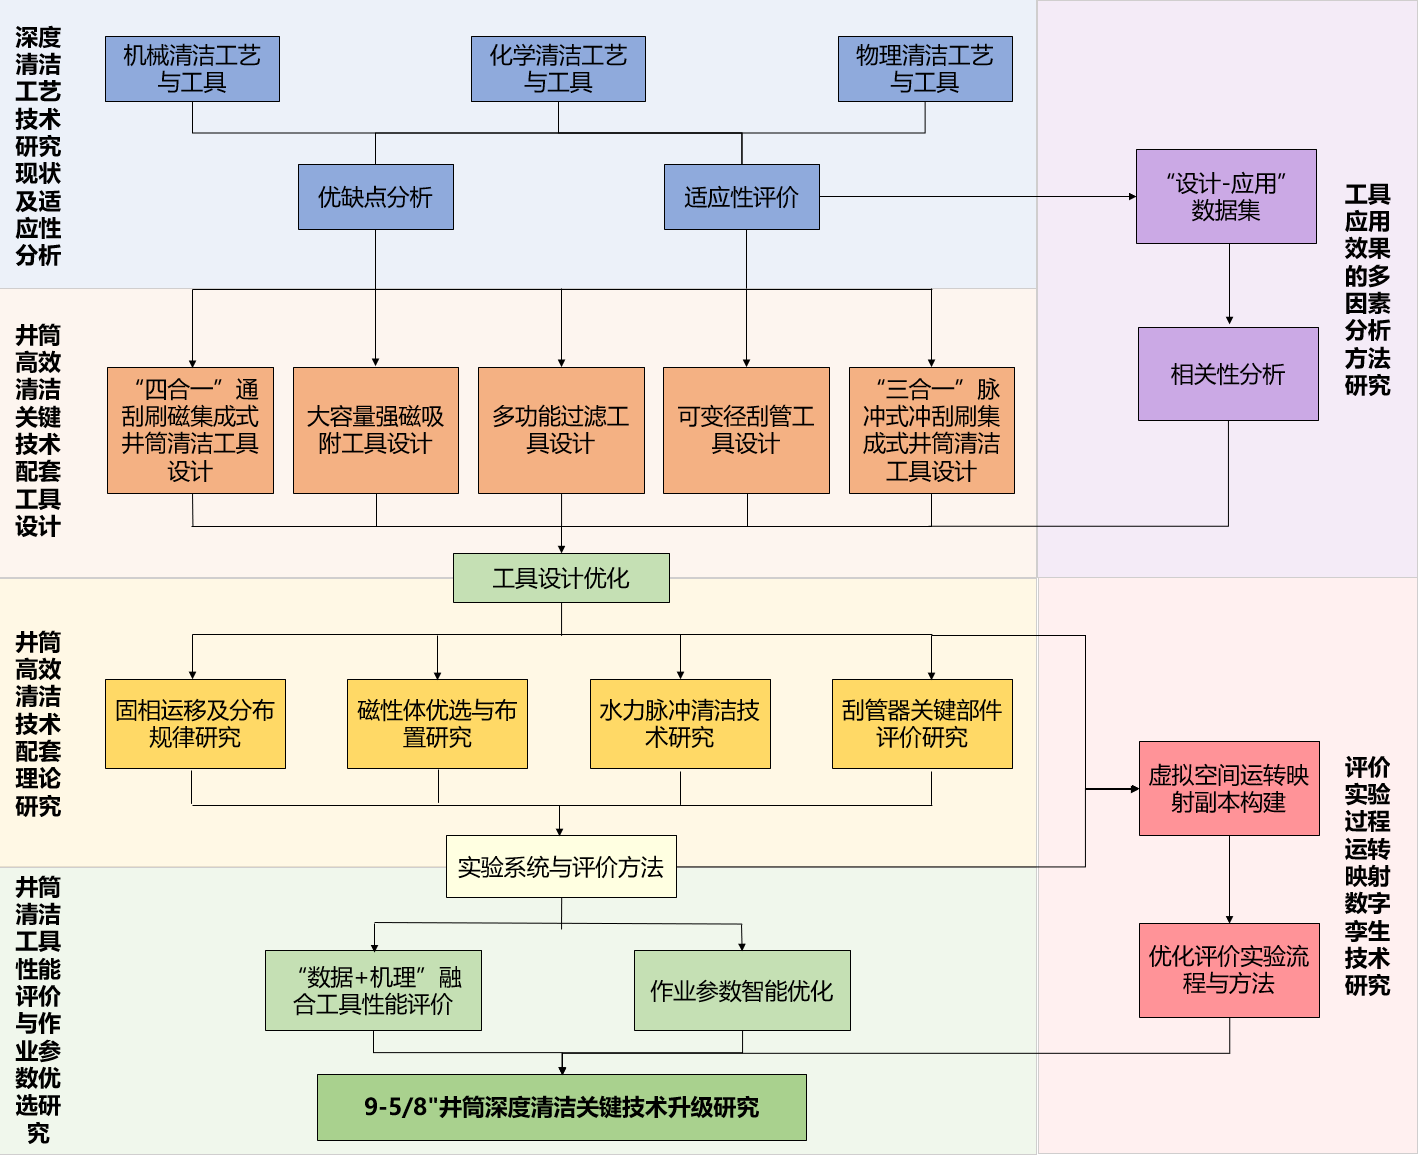
\includegraphics[width=0.98\textwidth]{figure/survey/tech-route.png}
	\caption{9-5/8\inch 井筒深度清洁关键技术总体技术路线}
	\label{fig:tech-route}
\end{figure}

按此路线，本报告后续内容安排如下：第 2 章以数值模拟揭示砂砾、铁屑、结垢物与蜡在井筒内的运移及分布规律，为工具结构与工艺参数提供理论依据；第 3 章依托全尺寸模拟实验台开展颗粒运移实验，验证并修正数值模型；第 4 章完成“三合一”“四合一”集成式工具、大容量强磁工具、多功能过滤工具与可变径刮管工具的结构设计、仿真校核与使用维护要求；第 5 章通过现场数据与室内实验数据的多因素分析，识别工具应用效果的主控因素；第 6 章建立工具性能评价方法与作业参数优选模型；第 7 章探索评价实验过程运转的数字孪生映射，为评价手段的智能化提供支撑。
